\documentclass[12pt,a4paper]{article}
\usepackage[utf8]{inputenc}
\usepackage[T1]{fontenc}
\usepackage{geometry}
\usepackage{titlesec}
\usepackage{hyperref}
\usepackage{graphicx}
\usepackage{fancyhdr}
\usepackage{enumitem}
\usepackage{tabularx}
\usepackage{float}
\geometry{left=2.5cm,right=2.5cm,top=2.5cm,bottom=2.5cm}

\title{\textbf{Renewal \& Upsell Advisor: System Workflow \& Architecture}}
\author{Demo Architecture Overview}
\date{\today}

\begin{document}

\maketitle

\section{Introduction}
This document outlines the high-level architecture and user flow for the Renewal \& Upsell Advisor platform. The platform is designed to ingest customer data, generate predictive insights using Machine Learning, and act upon those insights via automated Voice and Email agents.

\section{User Journey \& Data Flow}

\subsection{1. Onboarding \& Data Integration}
\begin{itemize}
    \item \textbf{Sign-in \& Authentication:} The user (e.g., a Customer Success Manager) signs into the platform securely.
    \item \textbf{Data Ingestion:} The user connects their database or uploads historical customer data via CSV/Excel formats. 
    \item \textbf{Synchronization:} The platform maps the ingested records (ARR, contract dates, licenses used, interactions) into the standardized PostgreSQL database (Supabase).
\end{itemize}

\subsection{2. Customization \& ML Modeling}
\begin{itemize}
    \item \textbf{Custom Formulas:} Users can configure custom logic and weights (e.g., how importance is given to utilization vs. sentiment).
    \item \textbf{Predictive Analytics:} The backend Machine Learning pipeline processes the data. It calculates Relationship Scores, Health Scores, Churn Probability, and identifies Upsell/Expansion opportunities automatically.
    \item \textbf{Continuous Learning:} The ML pipeline runs on a scheduled basis (e.g., daily at 12:00 AM) or can be triggered manually to reflect the latest data.
\end{itemize}

\subsection{3. Automated Agent Execution}
\begin{itemize}
    \item \textbf{Voice Bot (AI Agent):} Based on identified risks or opportunities, the system can deploy conversational Voice Agents (via Twilio). These agents engage customers using dynamic scripts to discuss renewals or expansions, recording sentiments and transcripts in real-time.
    \item \textbf{Email Campaign Automation:} Similarly, customized emails can be automatically drafted and sent to accounts hitting specific milestones.
\end{itemize}

\subsection{4. Real-time Monitoring \& Alerts}
\begin{itemize}
    \item \textbf{WebSocket Integration:} The frontend dashboard leverages WebSockets to stream real-time updates to the CSM.
    \item \textbf{Live Call Status:} When a voice agent is speaking with a customer, the status, duration, and immediate post-call sentiment analysis are pushed to the UI instantly.
    \item \textbf{Actionable Alerts:} High churn risk accounts trigger immediate alerts so the human CSM can intervene when necessary.
\end{itemize}

\section{Architecture Diagram}
For a visual breakdown of this flow, please refer to the architecture diagram below, which illustrates the sequence from data upload to ML generation, agent execution, and real-time frontend updates.

\begin{figure}[H]
    \centering
    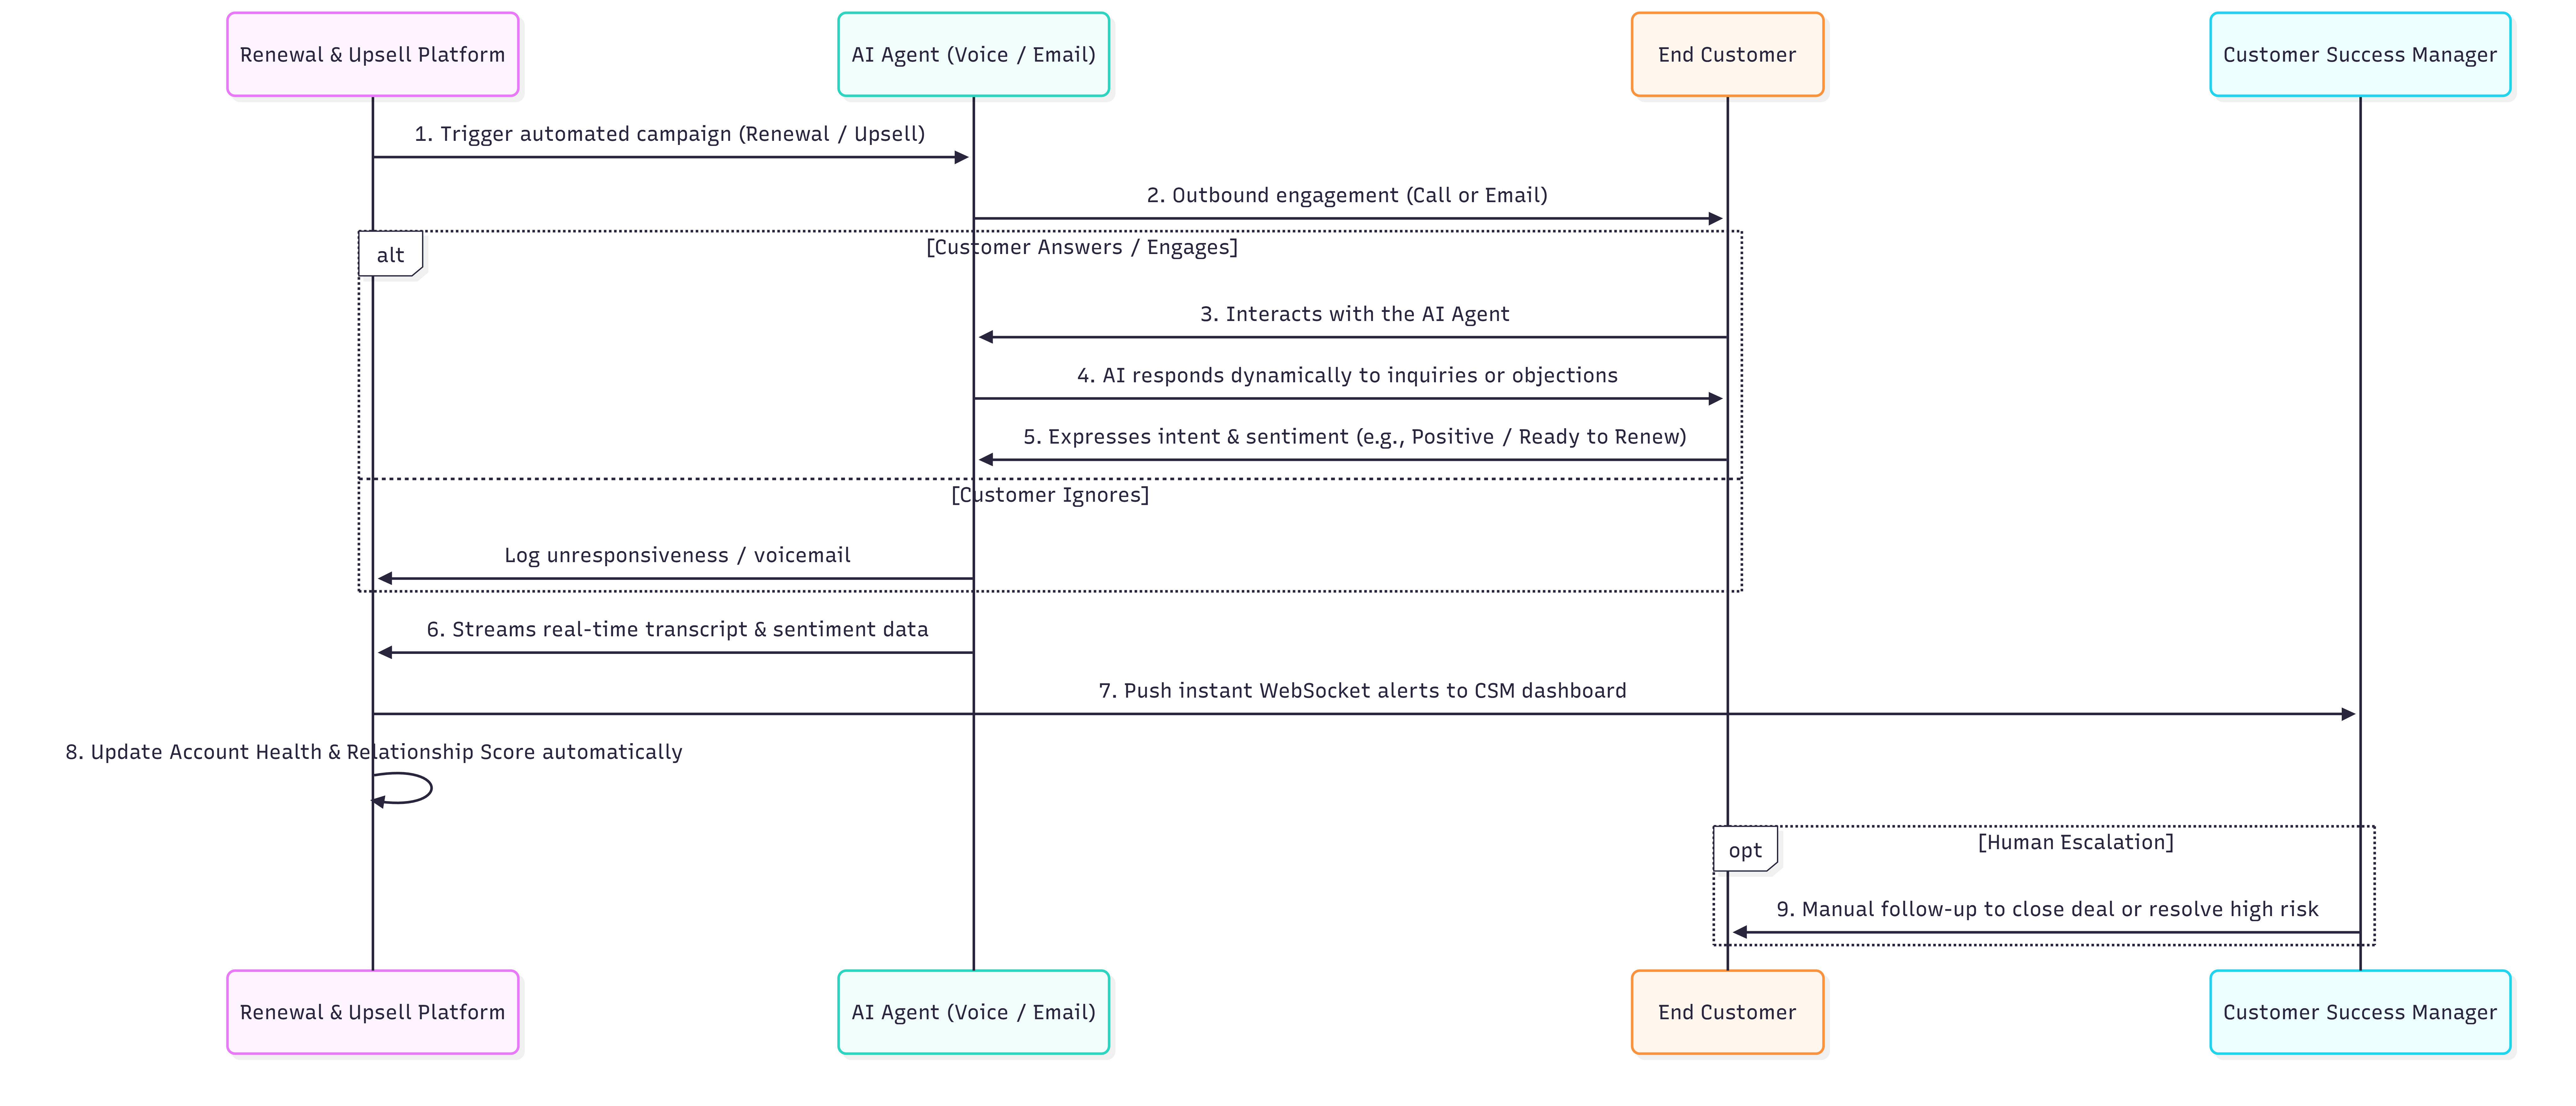
\includegraphics[width=\textwidth]{Demo.png}
    \caption{System Architecture \& Workflow}
    \label{fig:architecture}
\end{figure}

\section{Customer Agent Flow}
The following sequence details how the end-customer interacts with the AI Agents (Voice/Email) and how those interactions translate to live updates on the Customer Success Manager's dashboard.

\begin{figure}[H]
    \centering
    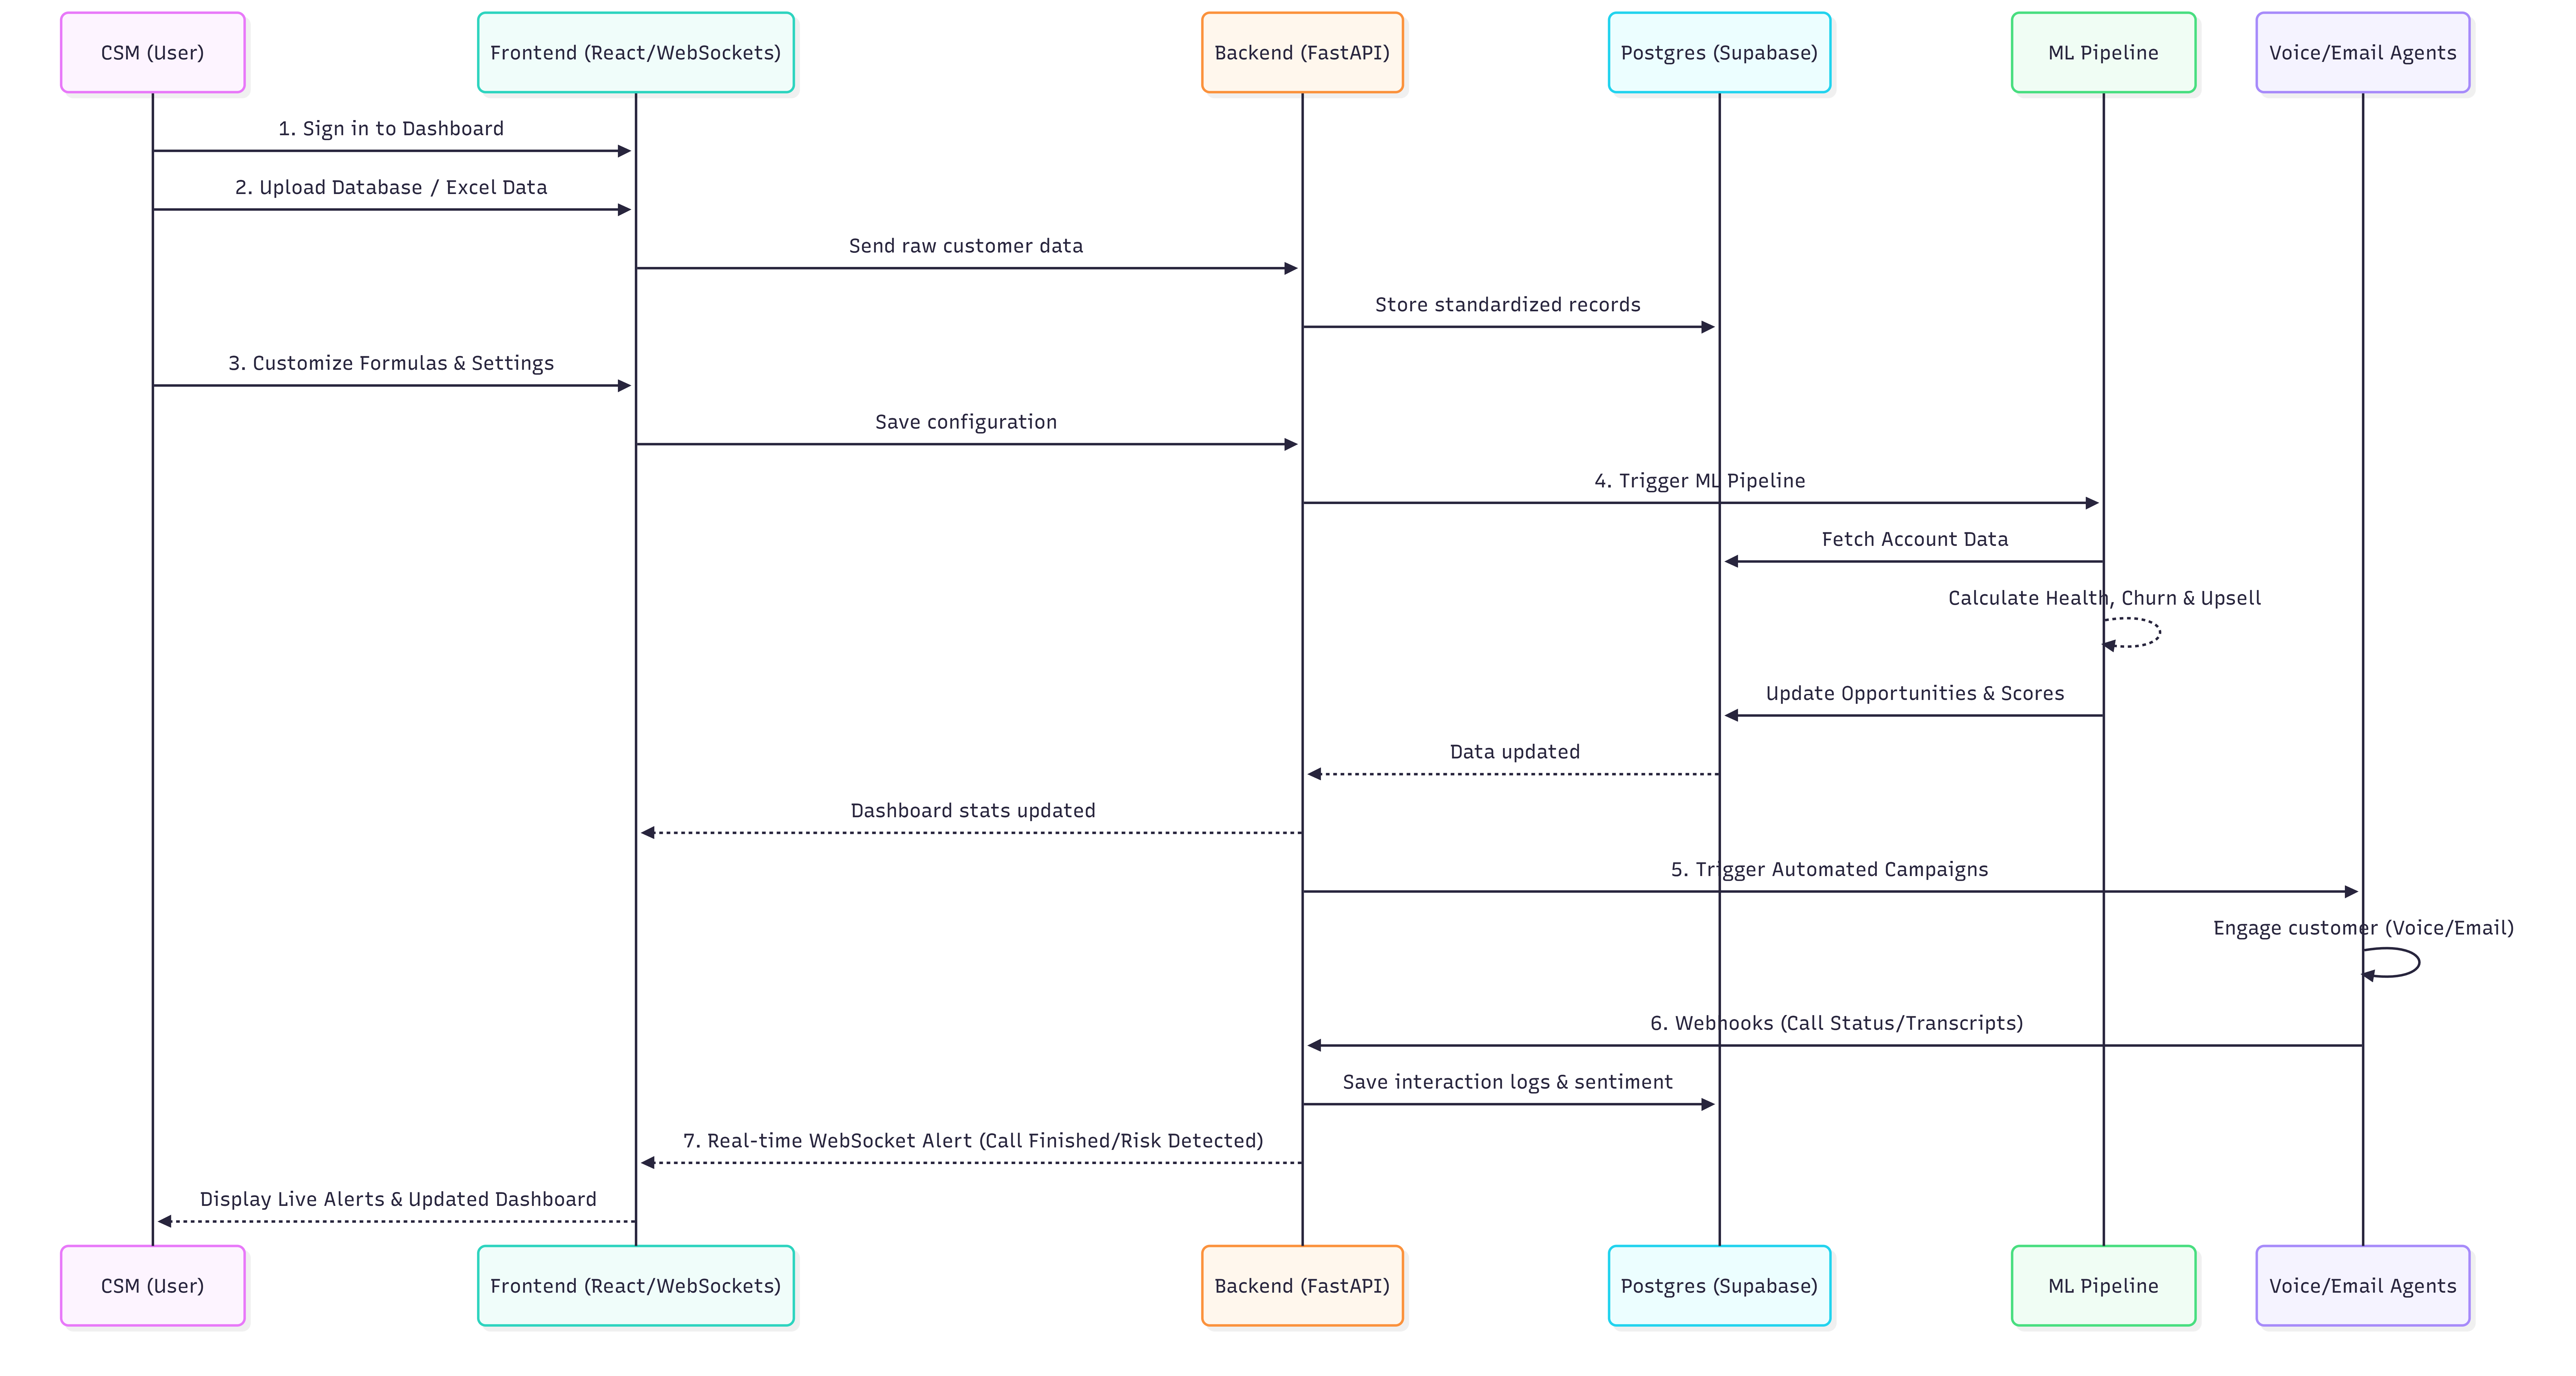
\includegraphics[width=\textwidth]{CustomerFlow.png}
    \caption{Automated Customer Engagement Flow}
    \label{fig:customer_flow}
\end{figure}

\end{document}
